\documentclass[journal]{IEEEtran}

% ---------- Engine & fonts ----------
\usepackage{iftex}
\ifXeTeX
  \usepackage{fontspec}
  % English fonts (TeX Gyre family)
  \setmainfont{TeX Gyre Termes}
  \setsansfont{TeX Gyre Heros}
  \setmonofont{TeX Gyre Cursor}
\fi

% ---------- Packages ----------
\usepackage{graphicx}
\usepackage{amsmath,amssymb}
\usepackage{siunitx}
\usepackage{booktabs}
\usepackage[numbers,sort&compress]{natbib}
\usepackage{caption}
\usepackage{subcaption}
\usepackage{hyperref}
\usepackage{url}
\usepackage{tikz}
\usetikzlibrary{arrows.meta,positioning,fit,calc}
\usepackage{pgfplots}
\pgfplotsset{compat=1.18}

% ---------- Helper: safe \input ----------
\makeatletter
\newcommand{\maybeinput}[1]{%
  \IfFileExists{#1}{\input{#1}}{\textit{[missing: #1]}}%
}
\makeatother

% ---------- Begin Document ----------
\begin{document}

\title{FeFET CMOS 0.18\,$\mu$m Integration Study}
\author{Samizo-AITL}
\maketitle

% ================= Abstract =================
\begin{abstract}
\maybeinput{build/abstract_en.tex}
\end{abstract}

\begin{IEEEkeywords}
FeFET, HfZrO$_x$, 0.18\,$\mu$m CMOS, reliability, process integration
\end{IEEEkeywords}

% ================= Body =================
\section{Introduction}
\maybeinput{build/intro_en.tex}

% =========================================================
% Process Integration
% =========================================================
\section{Process Integration}

\subsection*{Baseline and Added Steps}
The ferroelectric (FE) gate stack is inserted after polysilicon definition. 
Additional process steps are minimized and summarized in Table~\ref{tab:masks}. 
Fig.~\ref{fig:flow} shows placement within the baseline.

% ---- Flow (TikZ, vertical layout) ----
\begin{figure}[t]
\centering
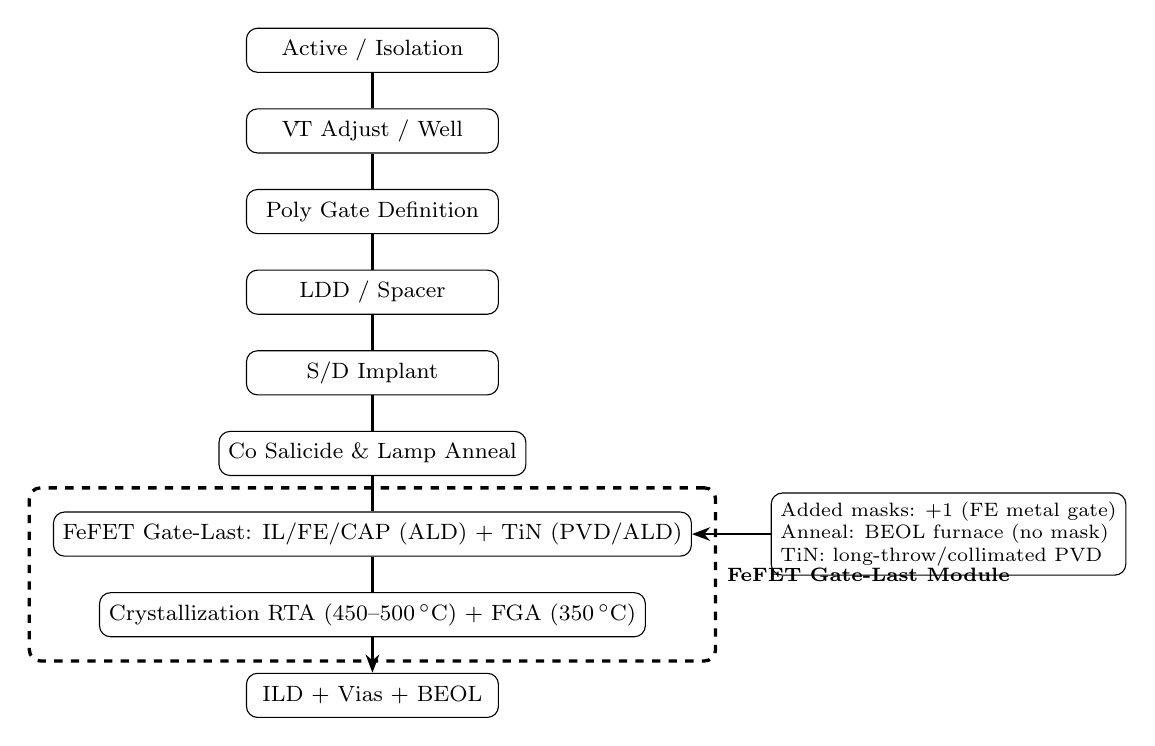
\begin{tikzpicture}[
  node distance=4.5mm,
  stage/.style={draw,rounded corners,minimum width=32mm,minimum height=5.6mm,align=center,font=\footnotesize},
  arr/.style={-{Stealth},thick},
  ann/.style={font=\scriptsize}
]
\node[stage] (act)  {Active / Isolation};
\node[stage,below=of act] (vt)  {V\!T Adjust / Well};
\node[stage,below=of vt]  (poly) {Poly Gate Definition};
\node[stage,below=of poly] (ldd)  {LDD / Spacer};
\node[stage,below=of ldd]  (imp)  {S/D Implant};
\node[stage,below=of imp]  (sal)  {Co Salicide \& Lamp Anneal};
\node[stage,below=of sal]  (fegate)  {FeFET Gate-Last: IL/FE/CAP (ALD) + TiN (PVD/ALD)};
\node[stage,below=of fegate]  (rta)  {Crystallization RTA (450--500\,\si{\celsius}) + FGA (350\,\si{\celsius})};
\node[stage,below=of rta]  (ild)  {ILD + Vias + BEOL};

\draw[arr] (act) -- (vt) -- (poly) -- (ldd) -- (imp) -- (sal) -- (fegate) -- (rta) -- (ild);

% dashed bracket to highlight FeFET module
\node[draw,dashed,very thick,rounded corners,fit=(fegate) (rta),inner sep=3mm,
      label={[ann]right:\textbf{FeFET Gate-Last Module}}] {};

% note box
\node[draw,rounded corners,align=left,font=\scriptsize,anchor=east,
      right=10mm of fegate] (note) {Added masks: +1 (FE metal gate)\\
Anneal: BEOL furnace (no mask)\\
TiN: long-throw/collimated PVD};
\draw[arr] (note.west) -- (fegate.east);
\end{tikzpicture}
\caption{Placement of FeFET module within the 0.18\,$\mu$m CMOS baseline (vertical layout).}
\label{fig:flow}
\end{figure}

% ---- Mask/step table ----
\begin{table}[t]
  \centering
  \caption{Added masks / process steps relative to baseline logic.}
  \label{tab:masks}
  \begin{tabular}{@{}lcc@{}}
    \toprule
    \textbf{Step} & \textbf{Mask} & \textbf{Comment}\\
    \midrule
    FE metal gate & +1 & Shared / reuse analog option route\\
    FE anneal     &  0 & Done in BEOL furnace (no extra mask)\\
    \bottomrule
  \end{tabular}
\end{table}

\subsection*{Device Stack}
TiN / Hf$_{0.5}$Zr$_{0.5}$O$_2$ (8--12\,nm, ALD) / Al$_2$O$_3$ IL (1--2\,nm) / p-Si.

\subsection*{Implementation Notes}
The 1.8\,V / 3.3\,V CMOS baseline was extended with an additional 1.8\,V FeFET option. 
FeFET devices are used as auxiliary elements for 1.8\,V SRAM macros, not as large-scale memory blocks. 
Although challenges remain regarding endurance, retention, TDDB, and yield, difficulty is reduced since large array scaling is not targeted. 
Integration is feasible within a legacy 0.18\,$\mu$m line by adding ALD; 
TiN can use existing barrier sputter (long-throw/collimated). 
The FeFET module is inserted after FEOL Co salicide and lamp anneal, requiring only one extra mask.

% =========================================================
% Experimental Conditions
% =========================================================
\section{Experimental Conditions}
\maybeinput{build/experimental_conditions_en.tex}

% =========================================================
% Reliability
% =========================================================
\section{Reliability}

% ---- Endurance (semilog cycles) ----
\begin{figure}[t]
\centering
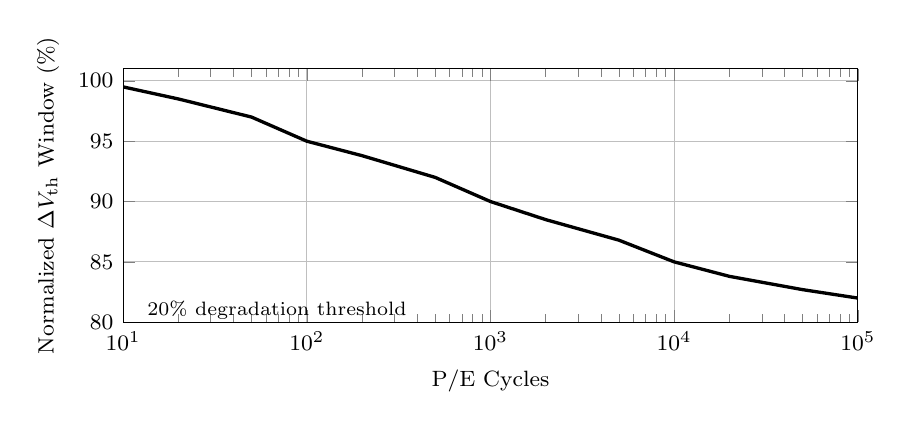
\begin{tikzpicture}
\begin{semilogxaxis}[
  width=0.9\linewidth,
  height=48mm,
  xmin=10, xmax=1e5,
  ymin=80, ymax=101,
  xlabel={P/E Cycles},
  ylabel={Normalized $\Delta V_{\mathrm{th}}$ Window (\%)},
  ymajorgrids, xmajorgrids,
  label style={font=\footnotesize},
  tick label style={font=\footnotesize},
]
\addplot[densely dashed] coordinates {(10,80) (1e5,80)};
\node[anchor=west,font=\scriptsize] at (axis cs:12,81) {20\% degradation threshold};
\addplot[very thick] table[row sep=\\]{
x   y\\
10  99.5\\
20  98.5\\
50  97.0\\
100 95.0\\
200 93.8\\
500 92.0\\
1000 90.0\\
2000 88.5\\
5000 86.8\\
10000 85.0\\
20000 83.8\\
50000 82.7\\
100000 82.0\\
};
\end{semilogxaxis}
\end{tikzpicture}
\caption{Endurance at $V_{\mathrm{PGM}}=2.5$\,V, pulse width $t=10$\,$\mu$s (illustrative trend).}
\label{fig:endurance}
\end{figure}

% ---- Wake-up + Retention subfigures ----
\begin{figure}[t]
\centering
\begin{subfigure}[b]{0.48\linewidth}
\centering
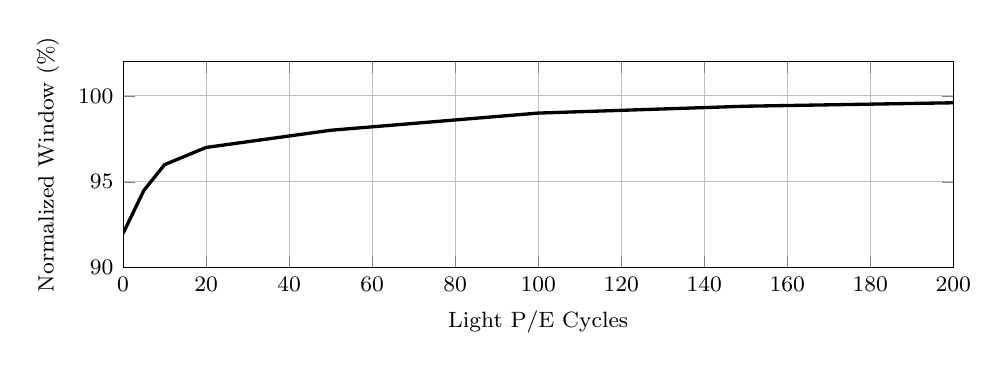
\begin{tikzpicture}
\begin{axis}[
  width=\linewidth, height=42mm,
  xmin=0, xmax=200,
  ymin=90, ymax=102,
  xlabel={Light P/E Cycles},
  ylabel={Normalized Window (\%)},
  ymajorgrids, xmajorgrids,
  label style={font=\footnotesize},
  tick label style={font=\footnotesize},
]
\addplot[very thick] table[row sep=\\]{
x  y\\
0  92.0\\
5  94.5\\
10 96.0\\
20 97.0\\
50 98.0\\
100 99.0\\
150 99.4\\
200 99.6\\
};
\end{axis}
\end{tikzpicture}
\caption{Wake-up: initial window increase.}
\end{subfigure}\hfill
\begin{subfigure}[b]{0.48\linewidth}
\centering
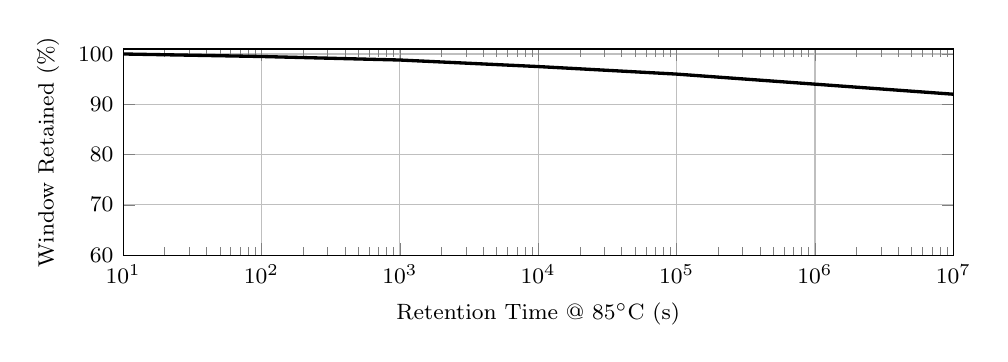
\begin{tikzpicture}
\begin{semilogxaxis}[
  width=\linewidth, height=42mm,
  xmin=1e1, xmax=1e7,
  ymin=60, ymax=101,
  xlabel={Retention Time @ 85$^\circ$C (s)},
  ylabel={Window Retained (\%)},
  ymajorgrids, xmajorgrids,
  label style={font=\footnotesize},
  tick label style={font=\footnotesize},
]
\addplot[very thick] table[row sep=\\]{
x     y\\
1e1   100\\
1e2   99.5\\
1e3   98.8\\
1e4   97.5\\
1e5   96.0\\
1e6   94.0\\
1e7   92.0\\
};
\end{semilogxaxis}
\end{tikzpicture}
\caption{Retention @ 85$^\circ$C (example extrapolation).}
\end{subfigure}
\caption{Wake-up and retention behaviors (illustrative).}
\end{figure}

% ---- TDDB (Weibull illustrative) ----
\begin{figure}[t]
\centering
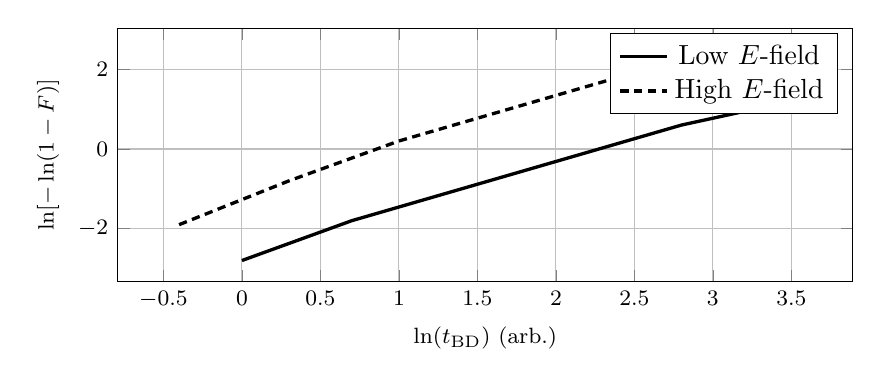
\begin{tikzpicture}
\begin{axis}[
  width=0.9\linewidth, height=48mm,
  xlabel={$\ln(t_{\mathrm{BD}})$ (arb.)},
  ylabel={$\ln[-\ln(1-F)]$},
  ymajorgrids, xmajorgrids,
  label style={font=\footnotesize},
  tick label style={font=\footnotesize},
]
% two stress conditions lines
\addplot[very thick] table[row sep=\\]{
x    y\\
0.0  -2.8\\
0.7  -1.8\\
1.4  -1.0\\
2.1  -0.2\\
2.8   0.6\\
3.5   1.2\\
};
\addlegendentry{Low $E$-field}
\addplot[densely dashed, very thick] table[row sep=\\]{
x    y\\
-0.4 -1.9\\
0.3  -0.8\\
1.0   0.2\\
1.7   1.0\\
2.4   1.8\\
3.1   2.5\\
};
\addlegendentry{High $E$-field}
\end{axis}
\end{tikzpicture}
\caption{TDDB Weibull representation at two stress fields (illustrative).}
\label{fig:tddb}
\end{figure}

\maybeinput{build/reliability_en.tex}

% =========================================================
% Conclusion
% =========================================================
\section{Conclusion}
\maybeinput{build/conclusion_en.tex}

% ================= References =================
\bibliographystyle{IEEEtran}
\bibliography{refs}

% ================= Biography =================
\section*{Author Biography}
Shinichi Samizo received the M.S. degree in Electrical and Electronic Engineering from Shinshu University, Japan.  
He joined Seiko Epson Corporation in 1997, where he engaged in semiconductor device process development including 0.25--0.18\,$\mu$m CMOS, HV-CMOS, \textbf{DRAM}, FeRAM, and FinFET/GAA research.  
He also contributed to inkjet MEMS process development and thin-film piezo actuator design, leading to the productization of PrecisionCore printheads.  
His expertise covers semiconductor devices (logic, memory \textbf{[DRAM/FeRAM/SRAM]}, high-voltage mixed integration), inkjet actuators, and AI-based control education.

\end{document}
